\subsection{Generated graphs} \label{results1}
To answer the first part of the research question, which is to compare the effects of no, global and local reallocation. For the simulation we chose to simulate 1000 time steps and use 30 simulations for each strategy. The regeneration rate of the sources is chosen randomly with the best rate being 10 times higher then the lowest. This is about in the range, that we found by analysing the amount of passengers at a train station per day. The number of colonies is chosen randomly between two and ten. Each of those colonies has 200 ants. We generated 30 different graphs and run our model on all of them. The simulation on many different graphs, with different regeneration rates and different amount of colonies should give us the ability to make a statistical statement about our results.

\begin{figure}[H]
	\centering
	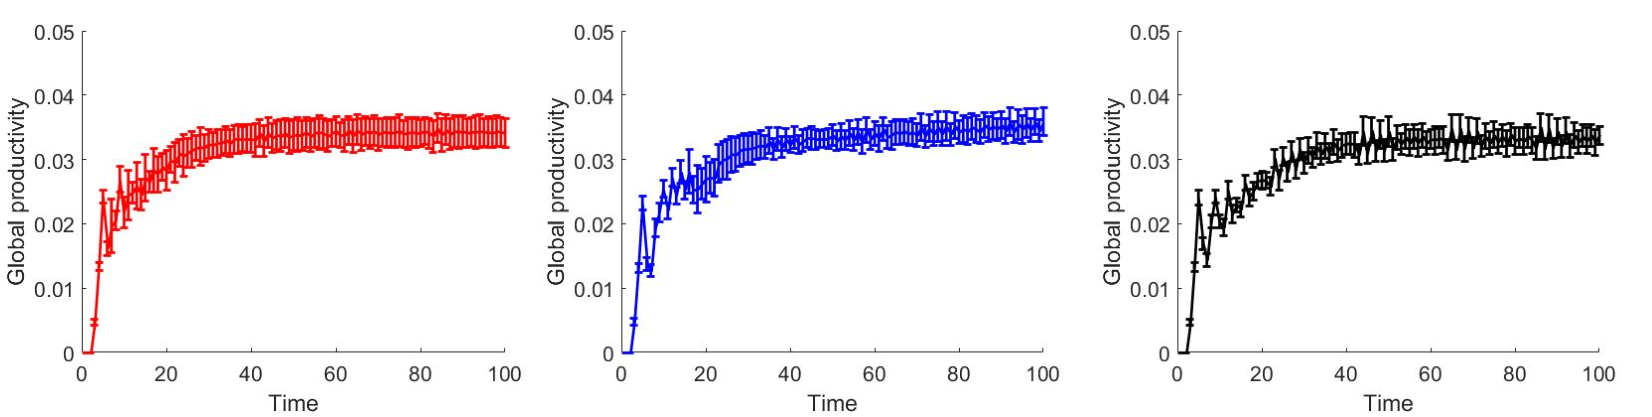
\includegraphics[scale=0.5]{globalProductivity.pdf}
	\caption{Plot of the global productivity of one graph using the above described parameters. The red line uses global reallocation, blue local and black does not use any reallocation.}
\end{figure}
The results of the simulations for each of the graphs looks very similar. The total productivity, which we wanted to optimize is very similar for all of the three strategies, and with the error margin being quite high it is not possible to draw the conclusion, that one of the strategies is better then the other ones. 
\subsubsection{Interpretation}
By looking at the amount of pheromones on the edges we assume the scenario, that every colony exploits a source, which is not used by the other colonies. This sign of cooperation shows, that the sources run low quickly and therefore the competition for a source is not worth. Note, that this is not the behaviour one would expect on a graph with only one colony and many food sources. In our example the ants are influenced by each other. Hence the solutions are not trivial like the ones in a simple one colony graph, which can easily be predicted. All colonies use this strategy and the sources are emptied quickly. Hence the reallocation of ants to a new colony does not have a great impact on the productivity, since the sources can not be exploited any more.

We suspect, that the results could be changed, with a modification of the parameters, like the number of ants per colony and most importantly the regeneration rate of the sources. The explanation, which is shown above would indicate, that the regeneration rate of the sources is low in comparison to the devaluation caused by the ants.

\subsection{SBB Network}
To answer the second question we ran our model on the SBB graph, We chose 2000 time steps, 5 train stations (the largest one in the SBB network) and 30 simulations for each strategy. The regeneration rate of the stations is chosen to match the total number of visitors per day of the stations. The results of the productivity have a strong similarity to the ones found with the random graphs. Again the error margin is very high and no conclusive results, supporting any of the strategies can be found. However when plotting the edges of the graph weighted by the amount of pheromones on them we can recreate the path taken by the ants.
\begin{figure}[H]
	\centering
	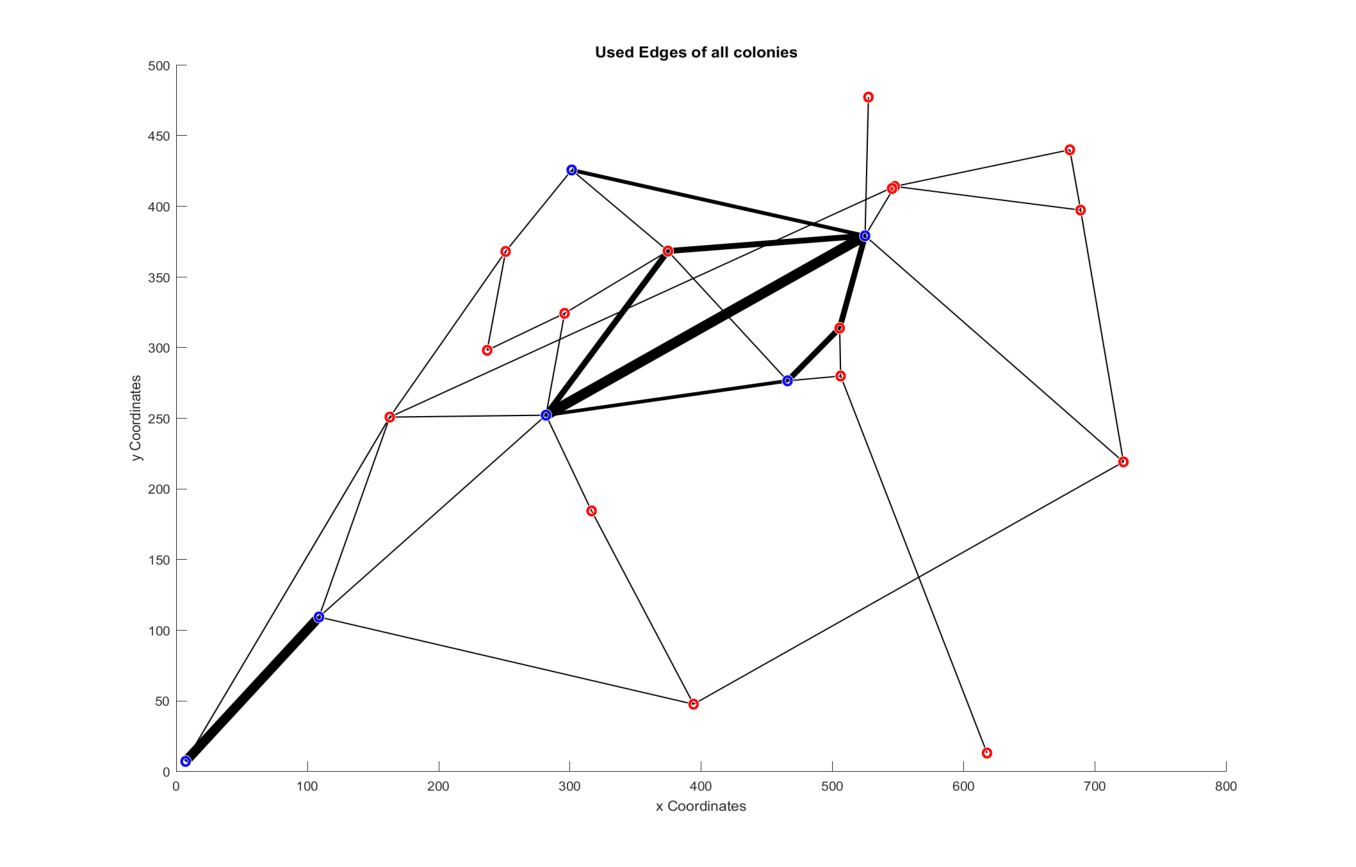
\includegraphics[scale=0.7]{sbbWeighted.pdf}
 	\caption{Graphic of the Swiss Rail Graph. The thickness of the edges represent the pheromone concentration.}
\end{figure}

\subsubsection{Interpretation}
We conclude, that for the parameters chosen the way, in which the trains are reallocated does not cause a statistically significant change in the productivity. However it is possible to identify the important connections to maximize the productivity. Since all of the strategies chose the same edges we assume, that those connections are essential for a high productivity in the network. This assumption is supported by an analysis from the SBB. In their map showing the passenger density of the different connections the graph shows a strong similarity to our predictions \citep{SbbStats4}. 